
\documentclass[bibtotocnumbered, headsepline,normalheadings,12pt,polish]{scrreprt}
\usepackage[T1]{fontenc}
\usepackage[utf8]{inputenc}
\usepackage{geometry}
\geometry{tmargin=25mm,bmargin=25mm,lmargin=30mm,rmargin=30mm}
\usepackage{babel}
\setlength\parindent{0pt}
\usepackage{graphics}
\usepackage{floatflt}
\usepackage{scrpage}
\usepackage{alltt}
\usepackage{pdfpages}
\usepackage{hyperref}
\usepackage{moreverb}

\pagestyle{headings}
\begin{document}
\title{\textbf{Dokumentacja iteracyjnego solvera rzadkich układów równań.}\\ \small{Projekt Języki i Metody Programowania I, Wydział Elektryczny}}
\author{Artur Skonecki \\ Prowadzący: dr inż. Jacek Starzyński}
\date{}
\maketitle


\tableofcontents

\chapter{Wstęp}
\section{Opis Problemu}
\normalsize
Macierze rzadkie często mają rozmiary, które uniemożliwiają lub czynią niepraktycznym rozwiązywanie ich przez algorytmy bezpośrednie. Metoda gradientów sprzężonych umożliwia rozwiązywanie układów równań liniowych. Ponieważ jest algorytmem iteracyjnym, metoda gradientów sprzężonych może by zastosowana do układów o rzadkich macierzach.
\\ \\
W celu zmniejszenia rozmiarów pamięci zajmowanej przez macierze , korzystnie jest zastosować algorytmy i struktury danych, które wykorzystają strukturę macierzy rzadkich. W prezentowanym programie wykorzystywany jest \texttt{schemat Yale}.
W schemacie Yale macierz przechowywana jest w 3 wektorach: \textbf{a, ia, ja}.\\

\normalsize
\begin{tabular}{| l || c | r |}
\hline
Element & Rozmiar & Opis \\
\hline
\hline
a  & ilość elementów niezerowych & wszystkie niezerowe wartości macierzy\\
\hline
ia & liczba kolumn + 1 & indeks pierwszego niezerowego elementu w wierszu\\
\hline
ja & ilość elementów niezerowych & pozycja kolumn niezerowych elementów\\
\hline
\end{tabular}

\section{Narzędzia}
\normalsize
Funkcja i program testowy zostały napisane w języku\texttt{ \textbf{C}} w standardzie \textbf{c8}9.
Wykorzystywano kompilator \textbf{gcc}, debugger \textbf{gdb} oraz testowano wycieki pamięci przy użyciu \textbf{valgrind} i \textbf{electric-fence}. Program budowano przy użyciu \textbf{GNU Make}. Dokumentacja zastała napisana w formacie \texttt{\textit{LaTeX}.}

\section{Format danych}
\normalsize
Jeżeli macierz nie jest kwadratowa to program testowy zakończy swoje działanie. Program wczytując macierze bierze pod uwagę tylko cyfry nad diagonalną, macierz pod diagonalną jest tworzona przez lustrzane odbicie. Wczytana macierz jest następnie zapisywana w formacie Yale.
Program wczytuje dane w następującym formacie:\\ \\
Przykładowa macierz.
\small
\begin{verbatim}
 6x6 [
3 0 0 1 0 3
0 3 1 4 5 6
0 0 3 0 0 0
0 0 0 3 0 0
0 0 0 0 3 1
0 0 0 0 0 3
]
\end{verbatim}



\chapter{Specyfikacja funkcjonalna}
\section{Solver}
\small
\verbatimtabinput[8]{man_solve}

\section{Program Testujący}
\small
\verbatimtabinput[8]{man_tester}

\chapter{Specyfikacja implementacyjna}
\section{Opis ogólny}
\normalsize
Krótki opis modułów.\\
\begin{tabular}{| l || c | c || r |}
\hline
MODUŁ & PLIKI & ZAWIERA & OPIS \\ \hline \hline
solver & solver.c solver.h & yale vec & zawiera funkcję rozwiązującą\\
main & main & tester define & punkt wejściowy programu\\
tester & tester.c tester.h & yale vec solver matrix define & moduł testujący\\
vec & vec.c vec.h & define & implementacja wektora\\
yale & yale.c yale.c & matrix vec define & implementacja schematu Yale\\
matrix & matrix.c matrix.hee & define & implementacja macierzy\\
define & define.h & - & stałe używane w programie\\
\hline
\end{tabular}
\\
\\ \\
Program korzysta z następujących systemowych plików nagłówkowych:
\begin{itemize}
\item stdlib.h
\item stdio.h
\item math.h
\item time.h
\end{itemize}

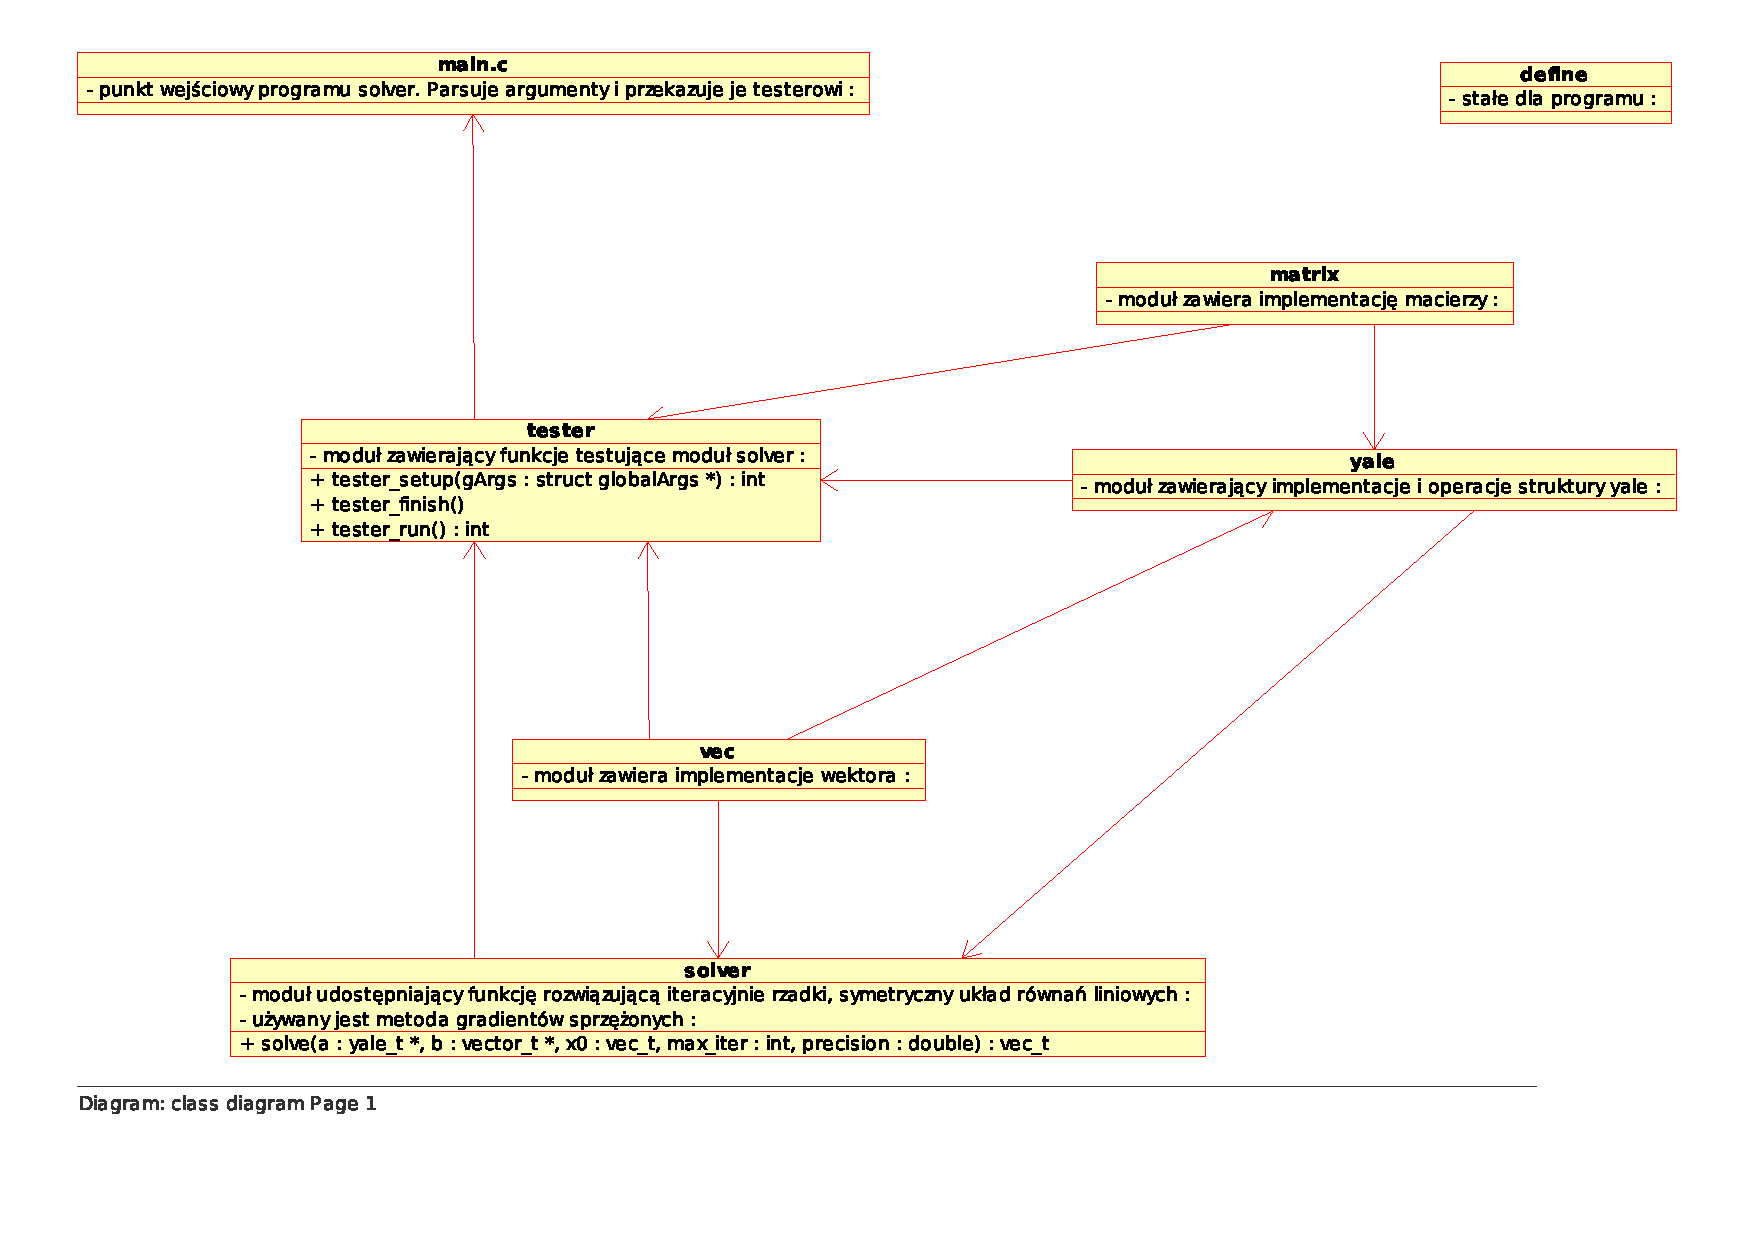
\includepdf[fitpaper,pages=1]{diagram_implement.pdf}
\section{Solver}
\subsection{Moduł solver}
\normalsize
Moduł \textbf{solver} składa się z 2 plików: \textit{\textbf{solver.c solver.h}} \\
W \textbf{solver} znajduje się implementacja funkcji rozwiązującej iteracyjnie rzadkie układy liniowe.
\textbf{solver} jest zależny od \large modułów \emph{vec i yale}.\normalsize\\
\noindent

Moduł solver udostępnia 1 funkcję:
\small
\begin{verbatim}
/* Funkcja rozwiązująca iteracyjnie rzadkie układy równań: 
   zwraca wskaźnik na wektor lub NULL w razie niepowodzenia */
vec_t solve (yale_t a, vec_t  b, vec_t  x0, int method, int max_iter, double precision)
\end{verbatim}
\normalsize
\begin{tabular}{| l | c | r |}
\hline
argument & typ & opis \\
\hline
a & yale\_t & macierz\\
b & vec\_t & wektor\\
x0 & vec\_t & wektor startowy\\
max\_iter & int & maksymalna liczba iteracjii\\
precision & double & dokładność wyniku\\
\hline
\end{tabular}

Funkcja \textbf{solve()} służy do rozwiązywania rzadkich układów liniowych. Wartość zwracana to wskaźnik na wektor wynikowy lub NULL w przypadku niepowodzenia.
Zastosowano \texttt{algorytm gradientów sprzężonych} ( \textit{conjugate gradients method} ).


\subsection{Moduł vec}
\normalsize
Moduł \textbf{vec} składa się z 2 plików: \textit{\textbf{vec.c vec.h}}\\
\textbf{vec} udostępnia prostą implementację wektora.\\
\textbf{vec} nie zależy od innych modułów. Potrzebuje jedynie plik \large\emph{define.h}.\normalsize\\

\textbf{vec} składa się z następujących elementów:
\small
\begin{verbatim}

typedef struct
{
    int n;      /* liczba elementow */
    double *p;  /* tablica elementow */
}*vec_t;

/* Funkcja porównuje dwa wektory: 
   zwraca TRUE lub FALSE gdy wektory są inne */
bool vec_cmp (vec_t  a, vec_t  b, double precision);

/* Funkcja generująca losowa wektor: 
   zwraca wskaźnik na wektor lub NULL w razie niepowodzenia */
vec_t vec_gen (int size, double ra, double rb, int pattern);

/* Funkcja wylicza normę wektora */
double vec_norm (vec_t  a);

/* Funkcja kopiująca wektor: 
   zwraca wskaźnik na wektor lub NULL w razie niepowodzenia */
vec_t vec_copy (vec_t  a);

/* Funkcja wczytująca wektor ze strumienia: 
   zwraca wskaźnik na wektor lub NULL w razie niepowodzenia */
vec_t wczytaj_vec (FILE *);

/* Funkcja wczytująca wektor ze pliku: 
   zwraca wskaźnik na wektor lub NULL w razie niepowodzenia */
vec_t wczytaj_vec_plik (char *);

/* Funkcja mnożąca 2 wektory */
double vec_mul (vec_t  a, vec_t  b);

/* Funkcja mnożąca wektor przez liczbę: 
   zwraca wskaźnik na wektor lub NULL w razie niepowodzenia */
vec_t vec_mul_val (vec_t  a, double val);

/* Funkcja dodająca wektor do wektora: 
   zwraca wskaźnik na wektor lub NULL w razie niepowodzenia */
vec_t vec_add (vec_t  a, vec_t  b);

/* Funkcja odejmująca wektor od wektora: 
   zwraca wskaźnik na wektor lub NULL w razie niepowodzenia */
vec_t vec_sub (vec_t  a, vec_t  b);

/* Funkcja pobiera z wektora element o indeksie i */
double vec_get (vec_t  a, int i);

/* Funkcja zapisuje wartość do wektora w indeksie i: 
   zwraca TRUE dla niepowodzenia  */
int vec_put (vec_t  a, int i, double x);

/* Funkcja mnożąca wektor przez liczbę: 
   zwraca wskaźnik na wektor lub NULL w razie niepowodzenia */
vec_t make_vec (int);

/*Funkcja uwalnia pamięć zaalokowaną dla wektora  */
void free_vec (vec_t  a);

/*Funkcja drukuje wektor do strumienia */
void print_vec (FILE * out, vec_t  a);
\end{verbatim}

\subsection{Moduł yale}
\normalsize
Moduł \textbf{yale} składa się z 2 plików: \textit{\textbf{tester.c tester.h}}\\
\textbf{yale} udostępnia minimalną implementację schematu Yale.\\
\textbf{yale} jest zależny od \large{modułów \emph{vec i matrix}}.\normalsize\\

\textbf{yale} składa się z następujących elementów.
\small
\begin{verbatim}

typedef struct yale
{
    double *a;  /* tablica z elementami niezerowymi */
    int *ia;    /* tablica z indeksami pierwszego niezerowego elementu w wierszu */
    int *ja;    /* tablica z kolumnami wszystkich niezerowych elementow*/
    int n;      /* liczba elementow niezerowych */
    int cols;   /* liczba kolumn */
} *yale_t;

/* Funkcja mnoży macierz yale przez wektor: 
   zwraca wskaźnik na wektor lub NULL w razie niepowodzenia*/
vec_t yale_mul_vec (yale_t y, vec_t  x0);

/* Funkcja konwertuje macierz matrix_t do yale_t: 
   zwraca wskaźnik na wektor lub NULL w razie niepowodzenia  */
yale_t make_yale (matrix_t  m);

/* Funkcja uwalnia pamięć zarezerwowaną dla struktury yale */
void free_yale (yale_t);

/* Funkcja alokuje pamięć dla struktury yale:
   zwraca wskaźnik na wektor lub NULL w razie niepowodzenia */ 
yale_t alloc_yale (int n, int ia_n);

/* Funkcja drukuje struktury yale w czytelny dla użytkownika sposób */
void print_yale (FILE * f, const yale_t y);

\end{verbatim}



\pagebreak

\section{Program Testujący}
\subsection{Moduł tester}
\normalsize
Moduł \textbf{tester} składa się z 2 plików: \textit{\textbf{tester.c tester.h}}\\
Zadaniem \textbf{tester}'a jest testowanie funkcji modułu \textbf{solver}.\\
tester jest zależny od \large{modułów \emph{vec, yale, matrix, solver}}.\normalsize\\
Udostępnia 3 funkcje i definicję struktury \textbf{globalArgs}, w której przechowywane są wszystkie parametry niezbędne \textbf{tester}'owi:\\
\small
\begin{verbatim}

struct globalArgs
{
    /* FLAGI */
    bool verbose;
    bool silent;
    bool nice_matrix;   /* losuj liczby całkowite */
    bool show_help;  
    bool m_static;      /* nie inicjuj generatora liczb losowych*/
    bool matrix_auto;   /* ignoruj dane wejściowe */

    char *outFile;      /* plik wyjściowy */
    char *matrix;       /* plik z macierza */
    char *matrix_x;     /* plik z wektorem wynikowym */
    char *matrix_x0;    /* plik z wektorem startowym */
    int m_size;         /* rozmiar losowanej macierzy */
    double m_sparsity;  /* rzadkość losowanej macierzy */
    double check;       /* dokładność porównywania macierzy 
                           wynikowej i wzoru */
    double precision;   /* dokładność do jakiej funkcji rozwiązującej */
    int max_iter;       /* maksymalna liczba iteracji */
    double range_min;   /* maksymalna losowana liczba */
    double range_max;   /* minimalna losowana liczba  */
    double diagonal;    /* wartost jakimi wypełniana jest diagonalna */
};

/* Funkcja wczytuje dane na podstawie struktury globalArgs: 
   w razie niepowodzenia zwraca prawdę */
int tester_setup (struct globalArgs *gArgs);

/* Funkcja uwalnia zasoby testera */
void tester_finish ();

/* Funkcja uruchamia tester: 
   w razie niepowodzenia zwraca prawdę */
int tester_run ();


\end{verbatim}


\subsection{Moduł matrix}
\normalsize
Moduł \textbf{matrix} składa się z 2 plików: \textit{\textbf{matrix.c} \textbf{matrix.h}}\\
Moduł \textbf{matrix} jest elementem pomocniczym używanym przez tester w celu wczytania lub losowego wygenerowania macierzy testowej.\\
\textbf{matrix} nie zależy od innych modułów. Potrzebuje jedynie plik \emph{define.h}.\\

Elementy modułu \textbf{matrix} potrzebne testerowi:
\small
\begin{verbatim}
typedef struct
{
    int rn; /* liczba kolumn */
    int cn; /* liczba wierszy
    double **p; /* 2 wymiarowa tablica z elemntami */
}*matrix_t;

/* Utworz nową macierz */
/* zwraca macierz lub NULL dla niepowodzenia */
matrix_t make_matrix (int, int);

/* Pobierz wartosc elementu */
double matrix_get (matrix_t  a, int i, int j);

/* wygeneruj losowo symetryczną macierz */
/* zwraca macierz lub NULL dla niepowodzenia */
matrix_t matrix_gen_sym (int size, double sparsity, double ra, double rb, int pattern);

/* zsymetryzuj macierz względem diagonalnej */
void matrix_symmetrize (matrix_t  a);

/* wczytaj macierz z pliku */
/* zwraca macierz lub NULL dla niepowodzenia */
matrix_t wczytaj_matrix_plik (char *);

/* wczytaj macierz ze strumienia */
/* zwraca macierz lub NULL dla niepowodzenia */
matrix_t wczytaj_matrix (FILE *);

/* drukuj macierz */
void print_matrix (FILE * out, matrix_t  a);

/* uwolniej zasoby macierzy */
void free_matrix (matrix_t  a);

\end{verbatim}
\subsection{Moduł main}
\normalsize
Moduł \textbf{main} składa się z 1 pliku: \textit{\textbf{main.c}}\\
Zadaniem \textbf{main} jest parsowanie argumentów lini poleceń przy użyciu biblioteki \textbf{getopt} i odpowiednie zapisanie ich w strukturze \textbf{globalArgs}, która zostaję następnie przekazana modułowi \textbf{tester}.
\textbf{main} jest zależny od \large{\emph{tester}}.\normalsize\\
\textbf{main} nie udostępnia żadnych funkcji.

\chapter{Testy}
\normalsize
\section{Kompilacja}
System operacyjny: Linux 2.6.24-21
Kompilator: gcc 4.2.4
\section{Wykorzystanie pamięci systemowej.}
Program testujący i funkcja \textbf{solve()} zostały przetestowane przy użyciu programu \textbf{valgrind} i b\textbf{iblioteki electric-fence}. Testy nie wykazały utraty pamięci.
\section{Program Testujący}
Funkcje matematyczne programu testującego zostały przetestowane przy użyciu programu \textbf{matlab}.
\section{Solver}
Przykładowe testy wykonywane na module \textbf{solver}: \\
\small
\begin{verbatim}
$ ./solver --verbose --sparsity 0.4 -min 0 --max 20  --diagonal 3.0
# losuj i rozwiązuj układ o rzadkości 0.4, liczbach z zakresu 0 20,
# wypełnij diagonalną 3.0, wyświetlaj maksymalną ilość informacji

$ ./solver -m data/m30x30 -x data/v30 --precision 1e-15
# wczytaj macierz i wektor wzorcowy, precyzja = 1e-15

$ ./solver --size 1000 --max-iter 2000 --sparsity 0.05 --quiet
# losuj macierz o rozmiarze 1000x1000, maksymalna liczba iteracji = 2000,
# rzadkość macierzy = 0.05, wyświetlaj minimalną ilość informacji

$ ./s ---nice --min -2000 --max 2000 --size 100 --diagonal 100
# losuj liczby całkowite z zakresu -2000 2000,
# rozmiar macierzy = 100, wypełnij diagonalną 100
\end{verbatim}
\normalsize
Przy dużych macierzach, macierzach o dużych liczbach i macierzach o małej rzadkości koniecznie jest zwiększenie liczby maksymalnej iteracji(domyślna 1000).


\begin{thebibliography}
\\

\bibitem{lh} \url{http://en.wikipedia.org/wiki/Sparse_matrix}
\bibitem{lh} \url{http://en.wikipedia.org/wiki/Conjugate_gradient_method}
\bibitem{lh} \url{http://www.inf.uni-konstanz.de/cgip/lehre/na_08/index.shtml.de}
\bibitem{lh} \url{http://www.icm.edu.pl/kdm/Metoda_gradient%C3%B3w_sprz%C4%99%C5%BConych_CG}
\bibitem{lh} \url{http://icis.pcz.pl/~roman/mat_dyd/zast_prz_rown/zrown.html}
\end{thebibliography}
\end{document} 
